\subsection{Continuity}\label{subsec-continuity}

\begin{definition}\label{def-continuity-at-point-a}
	Let $a\in\mathbb{R}$ and $\mathcal{D}\subset\mathbb{R}$. A function $f$ is
	continuous at the point $a$ if
	\begin{align}
		 & a\in\domain{f}\text{ and }\bigwedge_{\varepsilon>0}\bigvee_{\delta>0}\bigwedge_{x\in\domain{f}}
		\left(\abs{x-a}<\delta\implies\abs{f(x)-f(a)}<\varepsilon\right)\label{eq-continuity-at-point-a:1} \\
		\iff
		 & \lim_{x \to a}f(x) = f(a)\label{eq-continuity-at-point-a:2}                                     \\
		\iff
		 & \forall x_n \seqinfty{n} a \implies f(x_n) \seqinfty{n} f(a)\label{eq-continuity-at-point-a:3}
	\end{align}
\end{definition}

\begin{thm}\label{thm-elementary-functions-continuous}
	All elementary function in \pref{definition}{def-elementary-functions} are
	continuous everywhere in $a\in\domain{f}$.
\end{thm}

\begin{thm}\label{thm-arithmetic-continuous}
	The arithmetic operations defined in \pref{definition}{thm-limit-arithmetic}
	also preserve continuity.
\end{thm}

\begin{thm}\label{thm-composition-continuous}
	The composition of continuous function preserves continuity.
\end{thm}

\begin{proof}
	Of \pref{theorem}{thm-composition-continuous}.
	\begin{flushleft}
		The precise statement of this theorem goes as followed: If  $g$ is continuous
		at point $a$, and $f$ is continuous at $g(a)$, then $f \circ g$ is continuous
		at point $a$. So, by equation (\ref{eq-continuity-at-point-a:3}), let
		$x_n \seqinfty{n} a$. Then since $g$ is continuous at point $a$ and because $f$
		is continuous at $f(g(a))$, we can write
		\begin{align*}
			g(x_n)    & \seqinfty{n} g(a)    \\
			\implies
			f(g(x_n)) & \seqinfty{n} f(g(a))
		\end{align*}
		Hence, $f \circ g$ is continuous at $a$.
	\end{flushleft}
\end{proof}

\begin{definition}\label{def-one-sided-continuity}
	A function $f$ is continuous from the right side at the point $a$, if
	\begin{equation*}
		\lim_{a \to a^+} f(x)=f(a)
	\end{equation*}
	Similarly, $f$ is continuous from the left side at the point $a$, if
	\begin{equation*}
		\lim_{a \to a^-} f(x)=f(a)
	\end{equation*}
\end{definition}

\begin{exm}\label{exm-one-sided-continuity}
	The function $f(x)=\sqrt{x}$ is continuous from the right side at the point $0$,
	\textit{i.e.}
	\begin{equation*}
		\lim_{a \to 0^+} \sqrt{x}=0
	\end{equation*}
	but not from the left side because $\sqrt{x}$ is not defined for negative numbers.
	So, the square root function satisfies \pref{definition}{def-one-sided-continuity},
	but not \pref{definition}{def-continuity-at-point-a}. Therefore, $\sqrt{x}$ is
	only continuous on $[0,\infty)$.
\end{exm}

\begin{definition}\label{def-continuity}
	Moreover, we say a function is continuous \textit{iff} the function is continuous
	everywhere in $a\in\domain{f}$.
\end{definition}

\begin{rem}\label{rem-continuity}
	A function is continuous on $[a,b]$ if it is continuous on $(a,b)$ and satisfies
	both equations in \pref{definition}{def-one-sided-continuity}.
\end{rem}

\begin{definition}\label{def-removable-discontinuity}
	A function has a removable discontinuity if the limit of the function exists
	at the point $a$, but
	\begin{equation*}
		\lim_{x \to a}f(x)\neq f(a)
	\end{equation*}
	In some instances, $f(a)$ may not even by defined at all.
\end{definition}

\begin{exm}\label{exm-removable-discontinuity}
	Consider the function
	\begin{equation*}
		f(x)=\frac{\sin(x)}{x}
	\end{equation*}
	We saw in \pref{example}{exm-important-sin-over-x-limit} that
	\begin{equation*}
		\lim_{x\to0}\frac{\sin(x)}{x}=1
	\end{equation*}
	Notice that the function is not defined at $x=0$. To remove this discontinuity,
	we define a new function on top of the original one such that
	\begin{equation*}
		g(x)=\begin{cases}
			\frac{\sin(x)}{x}\text{ if }x\neq0 \\
			1\text{ if }x=0
		\end{cases}
	\end{equation*}
	Here, $g(x)$ fixes the discontinuity of $f(x)$.
\end{exm}

\begin{exm}\label{def-jump-discontinuity}
	A function has a jump discontinuity if both one-sided limits of the function
	exists, but
	\begin{equation*}
		\lim_{a \to a^+} f(x)\neq\lim_{a \to a^-} f(x)
	\end{equation*}
\end{exm}

\begin{exm}\label{exm-jump-discontinuity}
	Any step function has jump discontinuities, \textit{e.g.} the floor function
	defined in \pref{definition}{def-floor-function} or the ceiling function
	from \pref{definition}{def-ceiling-function}.
\end{exm}

\begin{definition}\label{def-infinite-discontinuity}
	A function has an infinite discontinuity\footnote{Sometimes also called an
		oscillating discontinuity} if at least one of the one-sided limits of $f$
	diverge.
\end{definition}

\begin{exm}\label{exm-infinite-discontinuity}
	Consider the function
	\begin{equation*}
		f(x)=\sin\left(\frac{1}{x}\right)
	\end{equation*}
	We saw in \pref{example}{exm-heine:1} that the limit at $x=0$ does not exists.
	So, $f$ has infinite discontinuities one the left-hand side and right-hand side.
\end{exm}

\begin{thm}\label{thm-monotone-jump-discontinuities}
	If a function $f$ is monotone on some interval, then $f$ only has jump discontinuities.
\end{thm}

\begin{thm}\label{thm-continuous-opposite-signs}
	Let $f:[a,b]\to\mathbb{R}$ be a continuous function. If $f(a)$ and $f(b)$ have
	opposite signs, then there exists a $c\in\mathbb{R}$ such that $f(c)=0$.
\end{thm}

\begin{proof}
	Proof of \pref{theorem}{thm-continuous-opposite-signs}.
	\begin{flushleft}
		\textbf{Answer:} The proof of this theorem involves an algorithm that is
		left to the reader as an exercise to implement. You can find more information
		about this online at \url{https://en.wikipedia.org/wiki/Bisection_method}.
	\end{flushleft}
\end{proof}

\begin{exm}\label{exm-continuous-opposite-signs:1}
	Let $p(x)=x^5-4x+1$. Show that this function has a root on the interval $[0,1]$.
	\begin{flushleft}
		\textbf{Answer}: By \pref{theorem}{thm-elementary-functions-continuous} this
		function is continuous $[0,1]$. Therefore we can use \pref{theorem}{thm-continuous-opposite-signs}
		to compute
		\begin{align*}
			 & p(0)=1>0, \\
			 & p(1)=-2<0 \\
		\end{align*}
		So, there exists a $c\in\mathbb{R}$ such that $p(c)=0$.
	\end{flushleft}
\end{exm}

\begin{rem}
	The mathematicians proved in the early \nth{19} century by \'Evariste Galois
	and Niels Henrik Abel separately that there is no closed formula to solve
	polynomials of degree $5$ and higher by using a combination of group theory
	and field theory, but the proofs itself are beyond the scope of this lecture
	because they are technically advanced.
\end{rem}

\begin{exm}\label{exm-continuous-opposite-signs:2}
	Show that the equation $\sin(x)=x-1$ has a solution.
	\begin{flushleft}
		\textbf{Answer}: Define the function
		\begin{equation*}
			f(x)=\sin(x)-x+1
		\end{equation*}
		Since $f$ is continuous on $[0,\pi]$ (\textit{cf.}
		\pref{figure}{sketch:exm-continuous-opposite-signs:2}), it follows that
		\begin{align*}
			 & f(0)=1>0,       \\
			 & f(\pi)=-\pi+1<0
		\end{align*}
		Therefore, by \pref{theorem}{thm-continuous-opposite-signs} there exists
		a $c\in\mathbb{R}$ such that $f(c)=0$.
	\end{flushleft}
	\begin{figure}[h!]
		\centering
		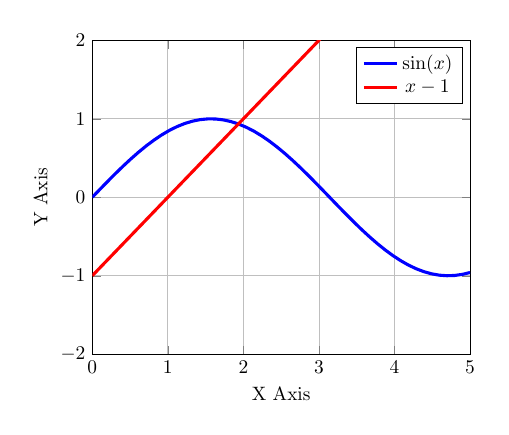
\begin{tikzpicture}[scale=0.7]
			\begin{axis}[
					xmax=5,
					xmin=0,
					ymax=2,
					ymin=-2,
					samples=50,
					grid=major,
					xlabel={X Axis},
					ylabel={Y Axis},
				]
				\addplot[blue, ultra thick,domain=0:5]{sin(deg(x))};
				\addplot[red, ultra thick,domain=0:5]{x-1};
				\legend{$\sin(x)$,$x-1$}
			\end{axis}
		\end{tikzpicture}
		\caption{Plot of the equation $\sin(x)=x-1$}
		\label{sketch:exm-continuous-opposite-signs:2}
	\end{figure}
\end{exm}

\begin{thm}\label{thm-intermediate-value-theorem}
	Let $f:[a,b]\to\mathbb{R}$ be a continuous function, and let $y_0$ be a value
	between $f(a)$ and $f(b)$. Then there exists an $x_0\in(a,b)$ such that
	\footnote{This a generalization of \pref{theorem}{thm-continuous-opposite-signs}}
	$f(x_0)=y_0$. \textit{Remark}: This theorem is also known as the intermediate
	value theorem.
\end{thm}

\begin{proof}
	Of \pref{theorem}{thm-intermediate-value-theorem}.
	\begin{flushleft}
		Assume \gls{wlog} that $f(a)<y_0<f(b)$. Then define $g(x)=f(x)-y_0$. By
		\pref{theorem}{thm-arithmetic-continuous} this function is also continuous on $[a,b]$.
		Therefore,
		\begin{align*}
			 & g(a)=f(a)-y_0<0, \\
			 & g(b)=f(b)-y_0>0
		\end{align*}
	\end{flushleft}
	By \pref{theorem}{thm-continuous-opposite-signs} there exists an $x_0$ such that
	$g(x_0)=0$. Therefore, $f(x_0)=y_0$.
\end{proof}

\begin{thm}\label{thm-weierstrass-theorems}
	Let $f:[a,b]\to\mathbb{R}$ be a continuous function. Weierstrass states the
	following two theorems:
	\begin{enumerate}
		\item The function $f$ is bounded.
		\item The function $f$ assumes a minimum and a maximum.
	\end{enumerate}
\end{thm}

\begin{thm}\label{thm-monotone-closed-interval}
	Let $f:[a,b]\to\mathbb{R}$ be a monotone function. Then, $f$ is continuous
	\textit{iff} the image of $f$ is a closed interval.
\end{thm}

\begin{proof}
	Of theorem (\ref{thm-monotone-closed-interval}).
	\begin{flushleft}
		By \pref{theorem}{thm-weierstrass-theorems}, statement 2, the function $f$
		assumes a minimum $m$ and maximum $M$. The image of $f$ is $[m,M]$ because
		$f$ obtains any value $y_0\in(m,M)$ by \pref{the intermediate value theorem}{thm-intermediate-value-theorem}.
	\end{flushleft}
\end{proof}

\begin{thm}\label{thm-continuous-monotone-invertible}
	If $f$ is continuous and strictly monotone, then $f$ is invertible whose
	inverse function is also continuous and monotone.
\end{thm}
